\documentclass{beamer}
\usetheme{Berkeley}
\usecolortheme{dolphin}
\title{Weekly Slides}
\author{K.~Tang\inst{1}}
\institute{
  \inst{1}
  Columbia University
}
\date{2012}

\begin{document}
\frame{\titlepage}

\section{October 3, 2012}
\begin{frame}
  \frametitle{SIFT fails to identify neural processes}
  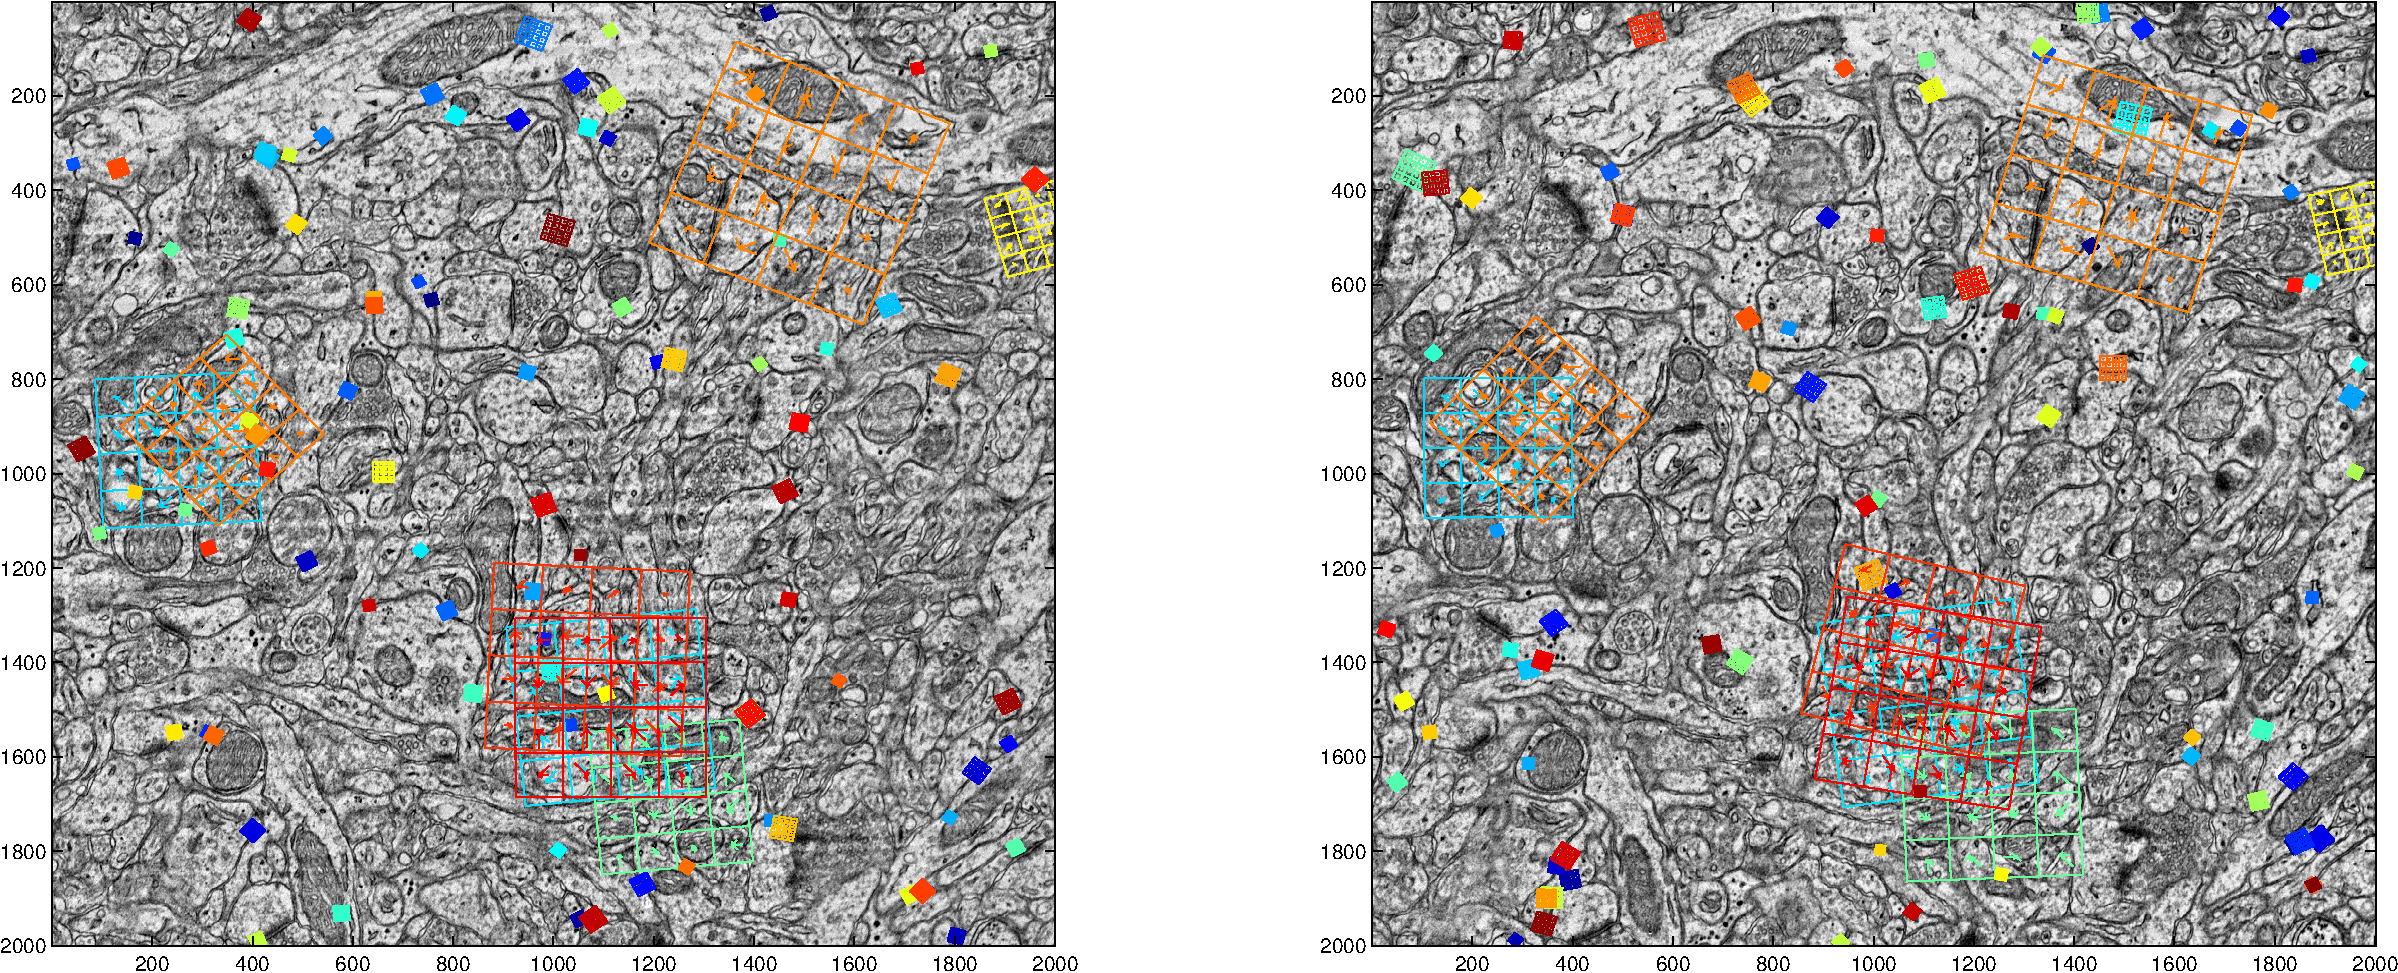
\includegraphics[width=\textwidth]{fig/sift_bock11}\\
  Two adjacent-depth images from the bock11 dataset \cite{Bock2011}. While large SIFT features are consistently transformed, small features move wildly. Thus SIFT is not appropriate for identifying neural processes.
\end{frame}

\section{References}
  \begin{frame}[allowframebreaks]
  \frametitle{References}
  \bibliographystyle{plain}
  \bibliography{refs.bib}
\end{frame}

\end{document}
